\chapter{Grundlagen}

\section{Container Technologie}

In der Vergangenheit verwendeten UNIX-ähnliche Betriebssysteme den Begriff Jail
("Gefängnis"), um eine modifizierte Programm Ausführungsumgebung zu beschreiben,
die Programme daran hinderte, auf geschützte Ressourcen zuzugreifen. Seit
2005, mit der Veröffentlichung davon Sun Solaris 10 und Solaris Containers, ist Container
der Begriff der Wahl für diese Art von Laufzeit. Das Ziel von besteht nicht
mehr darin, den Zugriff auf geschützte Ressourcen zu verhindern, sondern den Prozess
von allen Ressourcen zu isolieren, sofern dies nicht ausdrücklich erlaubt ist. Die
Verwendung von Containern ist seit langem eine bewährte Praxis. Das manuelle Erstellen
eines Containers kann jedoch schwierig sein und fehleranfällig. Die Industrie
verwendet derzeit die am weitesten verbreitete Container-Technologie Docker, um
das oben genannte Problem zu lösen.

\subsection{Docker Technologie}

Docker ist ein Befehlszeilenprogramm, ein Hintergrund Daemon und eine Reihe von
Remote Diensten, die logische Methoden verwenden, um allgemeine Softwareprobleme zu beheben und die Installation, Ausführung, Veröffentlichung und Deinstallation von Software mithilfe einer UNIX-Technologie namens Container zu vereinfachen.
Docker ist keine Programmiersprache oder ein Framework zur Softwareerstellung.
Dies ist OpenSourceLinuxSoftware, was bedeutet, dass jeder etwas beitragen kann
und dies aus einer anderen Sichtweise erfolgen muss. Ohne Docker verwenden
Unternehmen häufig Hardwarevirtualisierung (auch als Virtuelle Maschine (VM)
bekannt), um eine Isolierung zu erreichen. Die virtuelle Maschine stellt virtuelle
Hardware bereit, auf der Betriebssysteme und andere Software installiert werden
können. Die Erstellung dauert lange (meist wenige Minuten) und ist ressourcenintensiv, da sie neben der benötigten Software auch eine komplette Kopie des Betriebssystems ausführen. Anders als virtuelle Maschinen verwenden Docker-Container keine Hardwarevirtualisierung. Das im Docker-Container laufende Programm arbeitet direkt mit dem Linux-Kernel des Hosts zusammen. Er bietet eine sogenannte Abstraktion, sodass man sich im Fall von Docker nicht mit all den komplexen und spezifischen Aspekten der Installation einer Anwendung befasst werden muss, sondern nur mit der Software, die verwendet wird und somit ist der Einsatz dieser Technologie Zeit, Geld und Energie sparend \cite{Docker:overview}. 
Die folgende Abbildung veranschaulicht die Docker Architektur.

\begin{figure}[bth] 
	\centering
	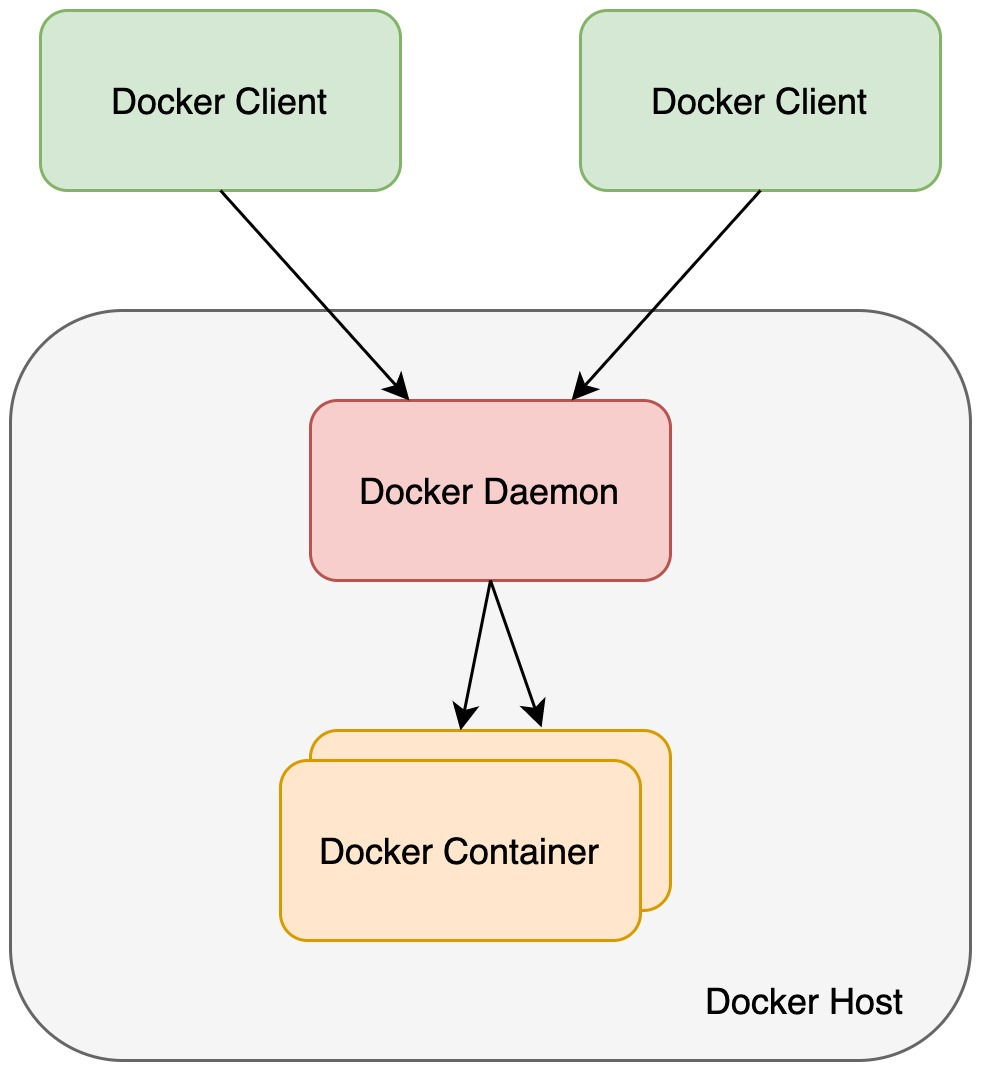
\includegraphics[width=0.5\textwidth]{Graphics/DockerArchitektur.png}
	\caption{Docker Architektur}
	%	\label{fig:cobus}
\end{figure}

\subsection{Kubernetes und dessen Aufbau}\label{sub-kubernetes}

Kubernetes ist ein Softwaresystem, das die Bereitstellung und Verwaltung von containerisierten Anwendungen vereinfacht. Es nutzt die Leistungsfähigkeit von Linux-Containern, um heterogene Anwendungen auszuführen, ohne die interne Struktur dieser Anwendungen verstehen und diese Anwendungen manuell auf jedem Host bereitstellen zu müssen. Da diese Anwendungen in Containern ausgeführt werden, wirken sie sich nicht auf andere Anwendungen aus, die auf demselben Server
ausgeführt werden. Die Anwendungen werden mit Docker-Technologie in Container
gekapselt, deshalb ist die Zusammenarbeit zwischen Kubernetes und Docker sehr wichtig. Mit Kubernetes kann die Software Anwendungen auf Tausenden von Computern Knoten ausgeführt werden, als ob alle diese Knoten ein riesiger Computer
wären. Es fasst die zugrunde liegende Infrastruktur zusammen und vereinfacht die Entwicklung, Bereitstellung und Verwaltung von Entwicklungs- und Betriebs-teams.
Unabhängig davon, ob der Cluster über einige wenige oder Tausende von Knoten verfügt, ist die Anwendungsbereitstellung auf Kubernetes immer gleich. Die Clustergröße macht keinen Unterschied. Die zusätzlichen Cluster knoten stellen nur
eine zusätzliche Menge verfügbarer Ressourcen für die bereitgestellte Anwendung
bereit \cite{kubernetes.io:concept}. 
\newline\newline
Ein Kubernetes-Cluster besteht aus vielen Knoten, die in zwei Typen unterteilt werden können: \textbf{Master Knoten}, der die Kubernetes-Steuerungsebene hostet, steuert und  verwaltet das gesamte Kubernetes-System.\textbf{Worker-Knoten} führen Ihre bereitgestellten Anwendungen aus. Die Nodes werden auf einem einzigen  Master-Node ausgeführt oder auf mehrere Nodes aufgeteilt und repliziert werden können, um eine hohe Verfügbarkeit zu erreichen \cite{kubernetes.io:concept}.
Kubernetes-Cluster besteht aus mehreren Komponenten, die von der Steuerungsebene gesteuert und verwaltet werden. Diese Komponenten sind zum einen, der Kubernetes API-Server, mit dem andere Komponenten der Steuerungsebene kommunizieren. Zum anderen ist der Scheduler, der die Anwendungen plant, der jeder verteilbaren Komponente der Anwendung einen Arbeitsknoten zuweist. Eine weitere Komponente ist der Controller-Manager, die Funktionen auf Cluster-Ebene ausführen, wie z. B. Komponenten duplizieren, Arbeitsknoten überwachen, Knoten Abfälle behandeln und
so weiter. Darüber hinaus besteht Kubernetes aus Etcd. Dies ist ein leistungsstarker verteilter Datenspeicher, der für permanente Speicherung der Cluster-Konfiguration
sorgt.

\begin{figure}[bth] 
	\centering
	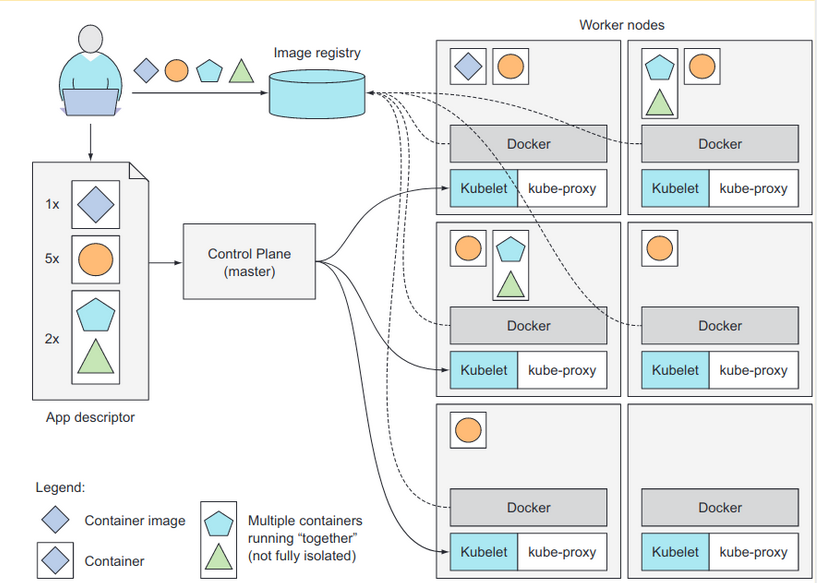
\includegraphics[width=0.7\textwidth]{Graphics/Kubernetes_Architektur.png}
	\caption{Kubernetes Architektur}
	%	\label{fig:cobus}
\end{figure}

\section{Einplatin Computer}

Der Begriff \ac{SBC} bezeichnet eine Prozessorplatine, die alle
vom Betriebssystem benötigten Komponenten wie Mikroprozessor, \ac{RAM}, Cache, Chipsatz usw. enthält. Mit zusätzlichen Aufsteckmodule können weitere Peripheriefunktionen für Ein- und Ausgabe, grafische Anzeige oder Kommunikationssteuerung ergänzt werden. Einplatinencomputer und Computer Module werden in industriellen, technischen, medizinischen und anderen kommerziellen Anwendungen wie Verkaufsautomaten oder Unterhaltungselektronik verwendet\cite{itwissen2017:raspi}.
Einer der beliebtesten und günstigsten Einplatinencomputer ist der Raspberry Pi, der von der britischen Raspberry Pi Foundation entwickelt wurde.
Der Raspberry Pi ist ein Minicomputer, der auf einer Platine von der Größe einer Kreditkarte montiert ist. Es wurde zu Schulungs- und Demonstrationszwecken entwickelt und ist vielseitig einsetzbar. An den Raspberry Pi können weitere Geräte angeschlossen oder Funktionen über USB, Ethernet oder 21 GPIO Pin-Schnittstellen gesteuert werden. Der Bildschirm kann über HDMI angeschlossen werden, um Grafik Inhalte in Full-HD-Qualität bis zu 1080p anzuzeigen. Der SD/MMC-Kartensteckplatz kann für das Betriebssystem verwendet werden und muss auf der Speicherkarte installiert werden. Darüber hinaus ist auch ein Erweiterungsmodul vorgesehen, mit dem beispielsweise eine drahtlose Verbindung über Bluetooth oder WLAN hergestellt werden kann. Ab Raspberry Pi 3 wurden Bluetooth und WLAN integriert. Typische Anwendungen von Raspberry Pi sind NAS- und VPN-Server, kleine Wohnzimmer-Mediacenter oder Smart-Home-Steuerung\cite{Cording2021:raspi}.

\section{Versionsverwaltungssystem}

Die Verwendung von \ac{VCS} für Softwareprojekte bietet mehrere Vorteile. \acs{VCS} ermöglicht es den Mitarbeitern, völlig frei mit dem Team zu arbeiten, sie können an jeder Datei arbeiten und sich jederzeit ohne Duplizierung gegenseitig Code überschreiben. Wenn zwei Entwickler Änderungen an derselben Datei vornehmen, führt \acs{VCS} die Änderungen zusammen oder warnt sie, dass ein Teil des Codes in Konflikt steht, da \acs{VCS} jede Änderung in der Datei oder im Code verfolgen kann und das gesamte Projekt in \acs{VCS} gespeichert wird. Da \acs{VCS} die Zusammenarbeit unterstützt, können Benutzer mit \acs{VCS} Daten, Dateien und Dokumente einfacher austauschen.
Eine wichtige Aufgabe besteht darin, die Version des Projekts nach Änderungen zu speichern. Das bedeutet, dass es immer auf eine bestimmte Version der Datei zugegriffen werden kann. \acs{VCS} ist sehr nützlich, da es die Möglichkeit bietet, versehentlich gelöschte oder bearbeitete Dateien wiederherzustellen\cite{Greene}.
Das \acs{VCS}-Repository enthält wichtige Informationen, die während des Entwicklungsprozesses verwendet werden können. Es ermöglicht auch, Speicherplatz sowohl auf dem Source Control
Client als auch auf dem Server zu sparen. Viele Unternehmen nutzen \acs{VCS} GitLab, um den Engineering-Teams, die Komplexität der Toolchain zu beseitigen und die Einführung von DevOps zu beschleunigen.

\section{Release Management}

Um bessere Dienste anbieten zu können, arbeiten viele Unternehmen hart daran,
neue Firmware, Fehlerbehebungen, Sicherheitsupdates und Leistungsverbesserungen
zu entwickeln. Dementsprechend hoffen viele Unternehmen, ihre schnellen Softwareentwicklungszyklen durch ein qualitativ hochwertiges Release-Management
zu unterstützen und zu verbessern. Release Management ist relativ neues Phänomen,
aber es ist eine sich schnell entwickelnde Disziplin im Software-Engineering. Dies dient dazu, die Integrität aufrechtzuerhalten und Betriebsunterbrechungen in IT-Umgebungen zu minimieren. Jedes Release wird unter Emergency Release, Minor Release und Major Release kategorisiert.

\subsection{Emergency Release}

Die Emergency Release zielt darauf ab, plötzlich auftretende oder dringende Probleme so schnell wie möglich zu lösen. Die Probleme Können schwerwiegende Fehler, die dazu führen, dass Teile der Software nicht mehr funktionieren oder kürzlich entdeckte Sicherheitslücken mit hoher Priorität sein.

\subsection{Minor Release}

Minor Release erweitert und verbessert bestehende Funktionen. Als weitere Funktion
kann Minor Release einen Emergency Fix ersetzen. Sie sind in der Regel kleiner als Major Release und nicht vollständig neue Versionen der Software, sondern aktualisiert vorhandener Software Version.

\subsection{Major Release}

Der größten Software Release ist der Major Release, die ebenso als neue Softwareversion bekannt ist. Der aktualisiert eine vorhandene Version einer Software. Normalerweise ersetzen sie vorherige Versionen der Software. Der Major Release enthält eine neu geschriebene Codebasis mit verbesserter Geschwindigkeit und Ausfallsicherheit. Er enthält auch Änderungen an der Benutzeroberfläche für ein neues Aussehen und die Integration mit neuer Software und/oder Kompatibilität mit neuerer Hardware.
Im Hinblick auf der Projekt-Release lassen sich Projekte in die folgenden zwei Strategien einteilen: 
\newline
Auf der einen Seite gibt es zukunftsorientierte Strategie. Ziel dieser Strategie ist es, Release zu erstellen, wenn bestimmte Bedingungen und Ziele erfüllt sind. Andererseits gibt es zeitbasierte Strategien – diese Strategie beinhaltet die
Festlegung eines bestimmten Release-Datums im Voraus und die Festlegung eines
Zeitplans, damit Entwickler entsprechend planen können. Es gibt eine Pre-Release-
Deadline, in der alle Features bewertet werden, um zu entscheiden, ob sie in die
Release aufgenommen werden können oder verzögert werden sollten.

\section{Typologien der Softwareverteilung}

Unter Softwareverteilung wird den Prozess der Softwareinstallation auf einem Computer
betrachtet. Während dieser Prozess auch im Serverbereich eine wichtige Rolle
spielt, ist er insgesamt sehr wichtig und die hohe Kundenzahl im Geschäft spiegelt
auch die Bedeutung dieses Prozesses in diesem Bereich wider. Die Verwendung der
automatischen Softwareverteilung hat mehrere Vorteile, einer der Vorteile ist der reduzierte
Verwaltungsaufwand und die progressive Installation. Es ist auch für eine
schnelle Systemaktualisierung, Systemwiederherstellung und Kostenreduzierung
von Vorteil. Sie ermöglicht auch die Installation außerhalb der Arbeitszeit.
Prinzipiell lassen sich drei Topologien für die Softwareverteilung voneinander unterscheiden.
\newline\newline
\textbf{Zentrale Softwareverteilung:} Bei der zentralisierten Softwareverteilung stellt nur 
ein Softwareverteilungsserver Dienste für alle Endpunkte bereit.
\newline
\textbf{Dezentrale Softwareverteilung:} Bei dezentralen Softwareverteilung erhält das Endgerät Software von mehreren Softwareverteilungsservern. 
Bestimmte Softwarepakete sind nur auf bestimmten Softwareverteilungsservern verfügbar.
\newline
\textbf{Hierarchische Softwareverteilung:} Bei der hierarchischen Softwareverteilung gibt es einen zentralen Softwareverteilungsserver, 
der Softwarepakete an mehrere untergeordnete Softwareverteilungsserver verteilt. 
Die Softwareverteilung verteilt Softwarepakete sequentiell von Geräten an Endpunkte. 
In dieser Topologie werden Aufgaben normalerweise auf verschiedenen Ebenen auf Softwareverteilungsserver verteilt. Orchestrierung und Paketieren erfolgen normalerweise an der Spitze der Server Hierarchie. Server auf niedrigerer Ebene werden nur verwendet, um Softwarepakete an Endpunkte zu verteilen \cite{FernandoBritoE:AbreuDaSilva}.